\section{Messungen mit Audio Precision (System Two Cascade)}
\subsection{Aufgabenstellung}
\begin{enumerate}
\item Messung des Quantisierungsrauschens (SNR) am Mischpult D/A Umsetzer (Line Ausgang des Lawo $mc^266$) mit $14-20$Bit Auflösung, Schrittweite 1 Bit. Vergleichen Sie mit den erwarteten werten. Was kann aus den Messergebnissen gefolgert werden?
\item Messung mit Jitter \begin{itemize}
\item Messung der FFT-Spektren verjitterter Signale. Untersuchung für verschiedene Jitterfrequenzen und verschiedene Signalfrequenzen.
\item Vergrößerung der Jitteramplitude, bis die Übertragung zusammenbricht.
\item Aufzeichnung der THD+N - Kennlinie bei Vergrößerung der Jitteramplitude bei den Jitterfrequenzen $500$Hz, $5$kHz und $10$kHz. 
\end{itemize}
\item Klirrfaktor (THD+N) und Rauschmessungen am Mischpult D/A-Umsetzer
\begin{itemize}
\item Messen einer THD+N-Kennlinie über den Dynamikbereich mit und ohne Dither
\item Messen einer THD+N-Kennlinie über der Frequenz mit und ohne Dither
\end{itemize}
\end{enumerate}
\subsection{Messaufbau}

\subsection{Formeln}

\subsection{Berechnungsbeispiele}

\subsection{Diagramme}

\subsubsection{Messung mit Jitter}

\begin{figure}
\centering
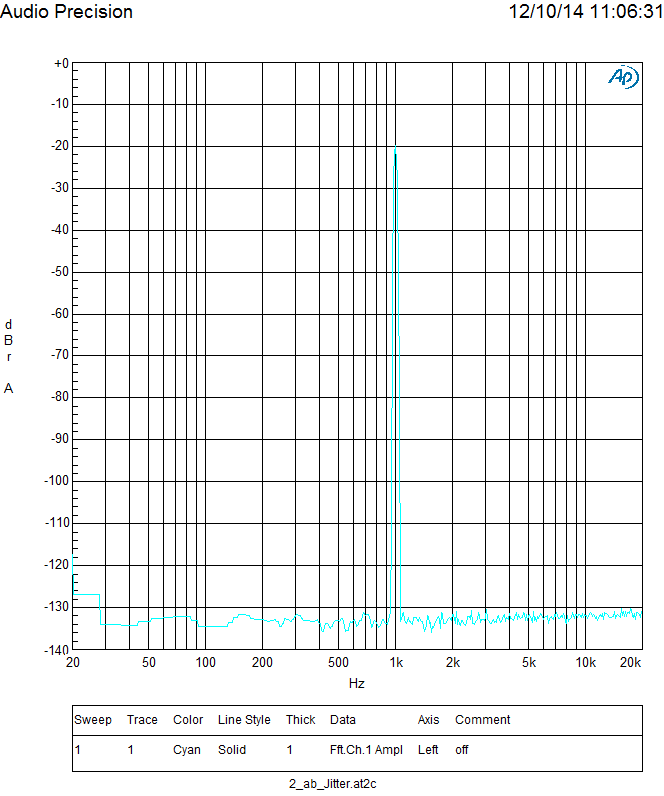
\includegraphics[width=\columnwidth]{figures/Aufg2/off_1khz.PNG} 
\caption{Test}
\end{figure}


\begin{figure}
\centering
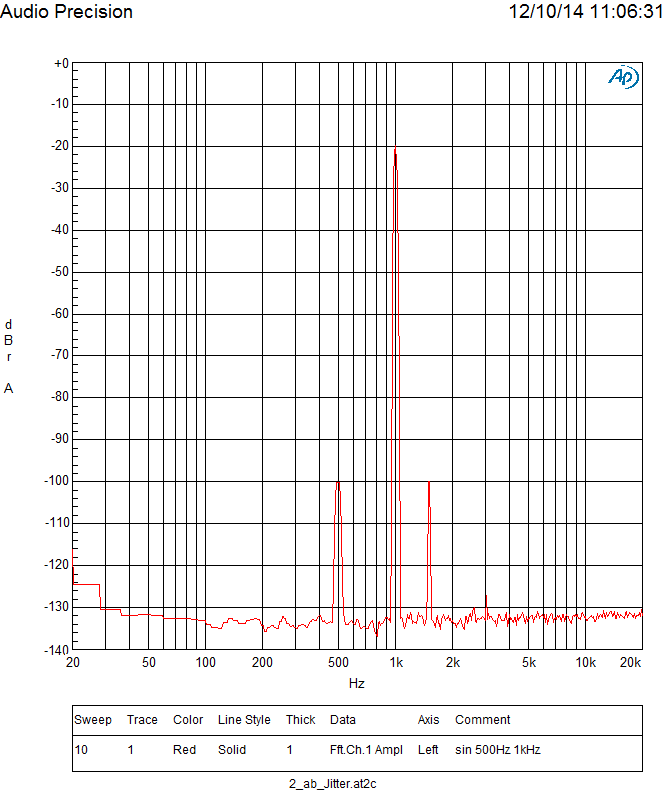
\includegraphics[width=\columnwidth]{figures/Aufg2/10.PNG} 
\caption{Test}
\end{figure}

\begin{figure}
\centering
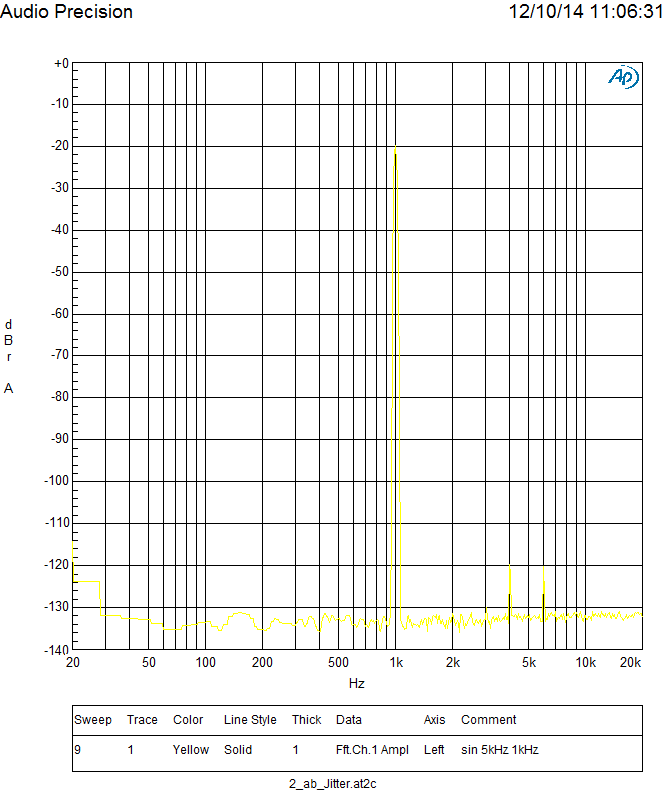
\includegraphics[width=\columnwidth]{figures/Aufg2/9.PNG} 
\caption{Test}
\end{figure}

\begin{figure}
\centering
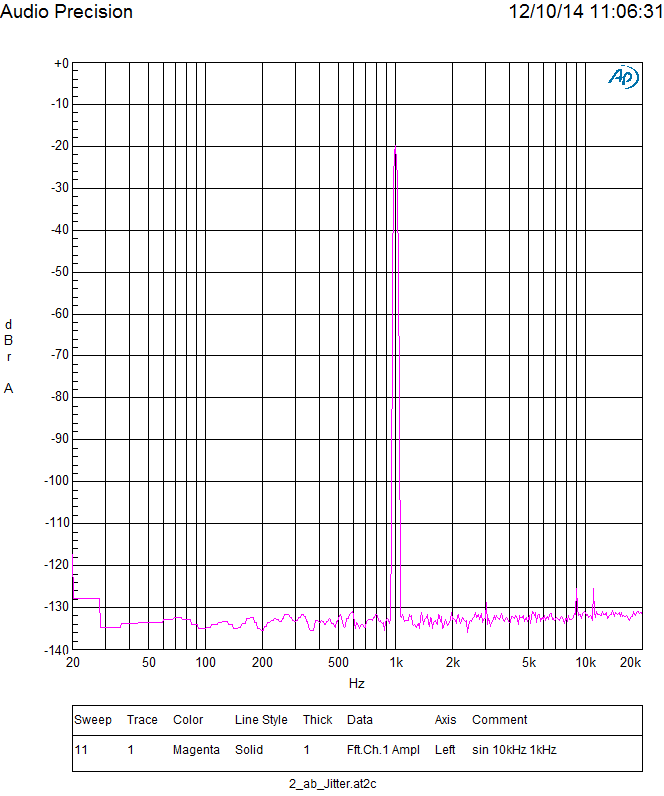
\includegraphics[width=\columnwidth]{figures/Aufg2/11.PNG} 
\caption{Test}
\end{figure}


\begin{figure}
\centering
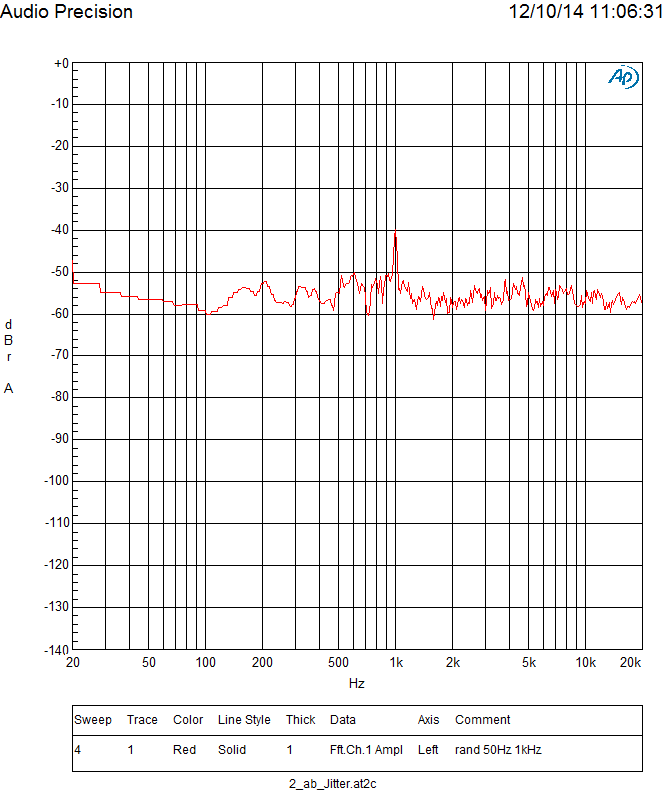
\includegraphics[width=\columnwidth]{figures/Aufg2/4.PNG} 
\caption{Test}
\end{figure}


%----------------------------------------------

\subsubsection{Klirrfaktor}


\begin{figure}
\centering
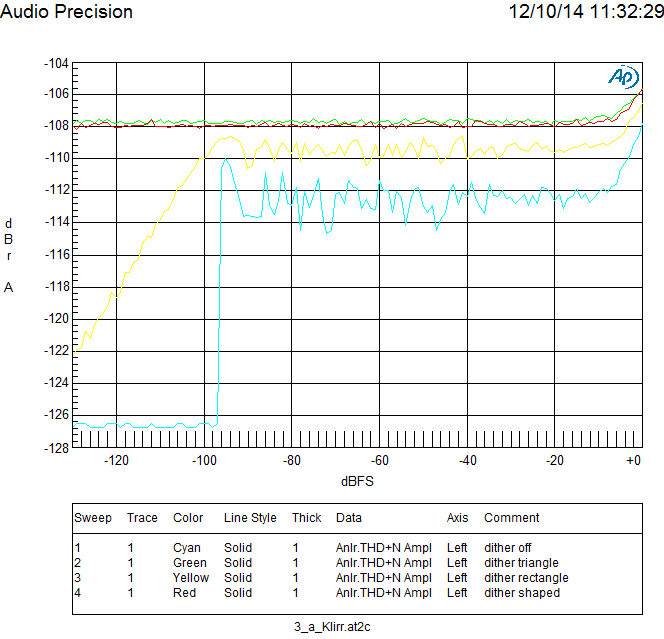
\includegraphics[width=\columnwidth]{figures/Aufg2/3a5.PNG} 
\caption{Test}
\end{figure}

\begin{figure}
\centering
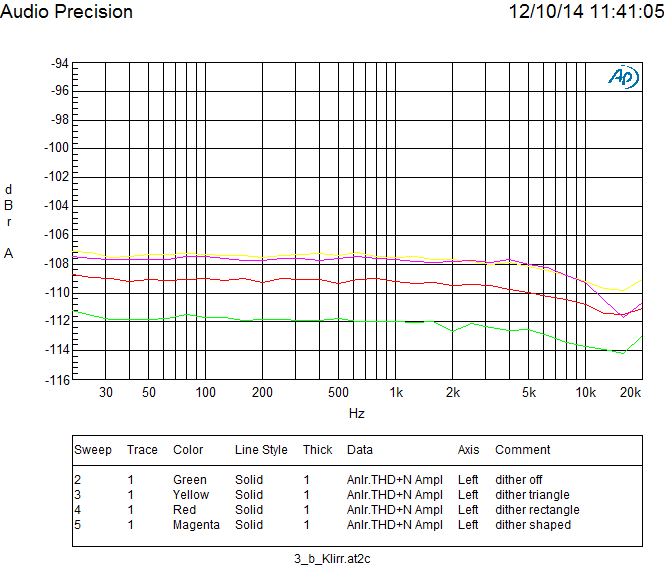
\includegraphics[width=\columnwidth]{figures/Aufg2/3b1.PNG} 
\caption{Test}
\end{figure}



\subsection{Geräteliste}

\subsection{Diskussion}

